\chapter{Experimental Setup}
The data used in this analysis were produced in $e^+e^-$ collisions at the KEKB accelerator and collected with the Belle detector. The experiment was hosted at the High Energy Accelerator Research Organization (KEK) in Tsukuba, Japan. The experiment ran
from years 1999 to 2010, collecting data at and near the energy of the $\Upsilon(4S)$ resonance. This chapter briefly describes the accelerator and the detector, based on detailed reports from \cite{doi:10.1093/ptep/pts102} and \cite{ABASHIAN2002117}, respectively.


\section{KEKB Accelerator}
KEKB is an asymmetric $e^+e^-$ collider, composed roughly of an electron source and a positron target, a linear accelerator (Linac) and two separate main rings with a circumference of about $3\e{km}$ as shown in Figure \ref{fig:kekb}. Electrons are first produced by a thermal electron gun and accelerated in the Linac to an energy of about $8\e{GeV}$. Part of the electrons collide with a tungsten target to produce positrons, which are accelerated in the Linac to an energy of about $3.5\e{GeV}$. Electron and positron beams are injected into the high- (HER) and low energy ring (LER) where they collide as bunches of particles at a single interaction point (IP) at an angle of about $22\e{mrad}$. The combined center-of-mass (CM) energy of the collision corresponds to the mass of the $\Upsilon(4S)$ resonance
\begin{equation}
E_{CM} = 2\sqrt{E_{e^+}E_{e^-}} = m_{\Upsilon(4S)}c^2 \approx 10.58\e{GeV}.
\end{equation}

\begin{figure}[H]
	\centering
	\captionsetup{width=0.8\linewidth}
	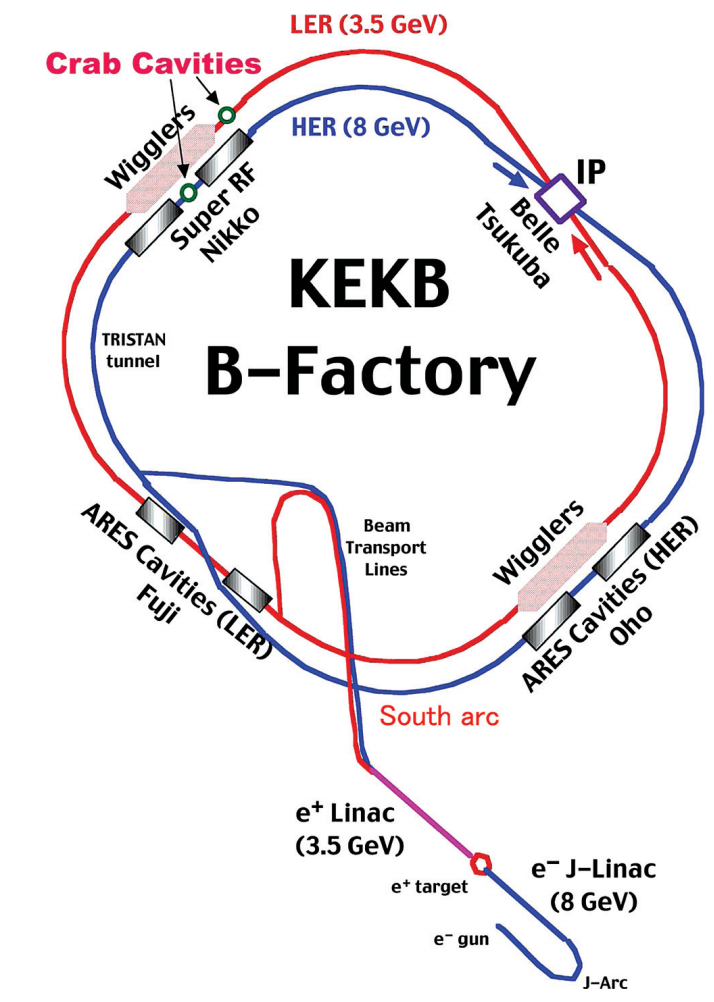
\includegraphics[width=0.5\linewidth]{fig/setup/KEKB}
	\caption{Schematic layout of the KEKB accelerator. The HER and the LER are the $e^-$ and the $e^+$ beams, respectively. Four experimental halls, FUJI, NIKKO, OHO and TSUKUBA are shown.}
	\label{fig:kekb}
\end{figure}

The $\Upsilon(4S)$ state is produced only in a fraction of all collisions, but when it is produced, it predominantly decays to a pair of charged or neutral $B$ mesons. This setup was chosen in accordance with the main goal of the experiment, which was to study CP
violation in the $B$ meson system. In other cases, the processes include $e^+e^-$ scattering, also known as Bhabha scattering, two-photon events, muon or tau lepton pair production, and production of $q \bar q$, where $q=u,\,d,\,s$ or $c$. Table \ref{tab:xsec} shows the cross-sections for all mentioned interactions in collisions of $e^+e^-$.
In addition to the nominal CM energy, the experiment collected data also at energies
corresponding to other $\Upsilon(nS)$ resonances, where $n = 1,\,2,\,3,\,5$, and also at energies below the resonances.

\begin{table}[H]
	\centering
	\begin{tabular}{|c|c|}
		\hline
		Interaction & Cross-section $[\mathrm{nb}]$ \\ 
		\hline
		$\Upsilon(4S) \to B \bar B$ & $1.2$ \\
		$q \bar q,~q \in [u,d,s,c]$ & $2.8$ \\
		$\mu^+\mu^-,~\tau^+\tau^-$ & $1.6$ \\
		Bhabha scattering (within detector acceptance)& $44$ \\
		Other QED processes (within detector acceptance)& $\sim 17$ \\
		\hline
		Total & $\sim 67$ \\
		\hline
	\end{tabular}
	\caption{Cross-sections with $L=10^{34}\e{cm^{-2}s^{-1}}$ for various physics processes at $\Upsilon(4S)$ resonance energy \cite{ABASHIAN2002117}.}
	\label{tab:xsec}
\end{table}

KEKB achieved the world-record for the peak luminosity of $2.11\E{34}\e{cm^{-2}s^{-1}}$, twice as much as the designed prediction, and the total integrated luminosity of $1041\e{fb^{-1}}$. Of the full Belle dataset, about $711\e{fb^{-1}}$ of data were taken at the $\Upsilon(4S)$ energy of $10.58\e{GeV}$, which corresponds to about $771\E{6}$ $B \bar B$ meson pairs.

\section{Belle Detector}
The Belle detector is a magnetic mass spectrometer which covers a large solid angle. It is designed to detect remnants of $e^+e^-$ collisions. The detector is configured around a $1.5\e{T}$ superconducting solenoid and iron structure surrounding the interaction point (IP). The 4-momentum of the decaying $B$ mesons and it's decayed daughter particles are determined via a series of sub-detector systems, which are installed in an onion-like shape. Short-lived particle decay vertices are measured by the silicon vertex detector (SVD) situated outside of a cylindrical beryllium beam pipe. Long-lived charged particle momentum is measured via tracking, which is performed by a wire drift chamber (CDC). Particle identification is provided by energy-loss measurements in CDC, aerogel Cherenkov counters (ACC) and time-of-flight counters (TOF), situated radially outside of CDC. Particles producing electromagnetic showers deposit energy in an array of CsI(Tl) crystals, known as the electromagnetic calorimeter (ECL), which is located inside the solenoid coil. Muons and $K_L$ mesons (KLM) are identified by arrays of resistive plate counters in the iron yoke on the outside of the coil. 

The coordinate system of the Belle detector originates at the IP, with the $z$ axis pointing in the opposite direction of the positron beam, the $x$ axis pointing horizontally out of the ring, and the $y$ axis being perpendicular to the aforementioned axes. Th electron beam crosses the positron beam at an angle of about $22^\circ$. The polar angle $\theta$ covers the region between $17^\circ \leq \theta \leq 150^\circ$, while the cylindrical angle $\varphi$ covers the full $360^\circ$ range, amounting to about $92\%$ coverage of the full solid angle.

%TODO: add detector image


%In our analysis, key features of the Belle detector are as follows.
%•
%Good particle detection efficiency for 4-
%π
%region to collect all the particles in an
%e
%+
%e
%−
%collision.  This is important not only for the good signal reconstruction efficiency,
%but also for background reduction since un-detected particles from various
%B
%decay
%modes are the main source of the background.
%•
%Good reconstruction efficiency for low-momentum particles.  Since decay particles
%from
%D
%∗
%mesons and
%τ
%leptons are produced in a chain of multi-body decays, their
%momenta are about 0.7 GeV
%/c
%on average and lower than 1.5 GeV
%/c
%.
%•
%Good  momentum  resolution  in  the  tracking  devices  and  energy  resolution  in  the
%ECL.
%•
%Good PID performance for charged particles.

%\subsection{Extreme forward calorimeter (EFC)}

\subsection{Silicon Vertex Detector}
SVD is the inner-most part of the Belle detector and serves the purpose of measuring the decay vertices of decaying particles. The precision of the subsystem is about $100\e{\mu m}$, which is important for measuring the difference in $z$-vertex positions of the $B$ mesons in time-dependent CP violation studies. The main parts of the SVD are the double-sided silicon detectors (DSSD). With their thin profile and parallel silicon strips on both sides they provide 2D hit information of charged particle and are perfect for a small-scale device which acts with high precision.

During the data taking period, two configurations of the SVD have been used. The first, SVD1, has three layers of DSSD detectors, positioned at $30$, $45.5$ and $60\e{mm}$ away from the IP. They compose a ladder-like structure, covering the polar angle of $23^\circ < \theta < 140^\circ$. This configuration was used from the beginning of the experiment until 2003 when a dataset of about $1.52\E{8}$ pairs of $B \bar B$ mesons were recorded. Due to problems with radiation hardness, a new configuration was used, SVD2, which was operational until the end of data taking, measuring about $6.20\E{8}$ pairs of $B \bar B$ mesons. The SVD2 has 4 layers of DSSD detectors positioned at $20$, $43.5$, $70$ and $80\e{mm}$ away from the IP and covered the polar angle of $17^\circ < \theta < 150^\circ$. The first layer was moved closer to the IP, which greatly improved the sub-system precision, due to multiple-Coulomb scattering affecting resolution more as the distance from the IP increases. The front and side view of the SVD2 are shown in Figure \ref{fig:SVD_layout}.

\begin{figure}[H]
	\centering
	\captionsetup{width=0.8\linewidth}
	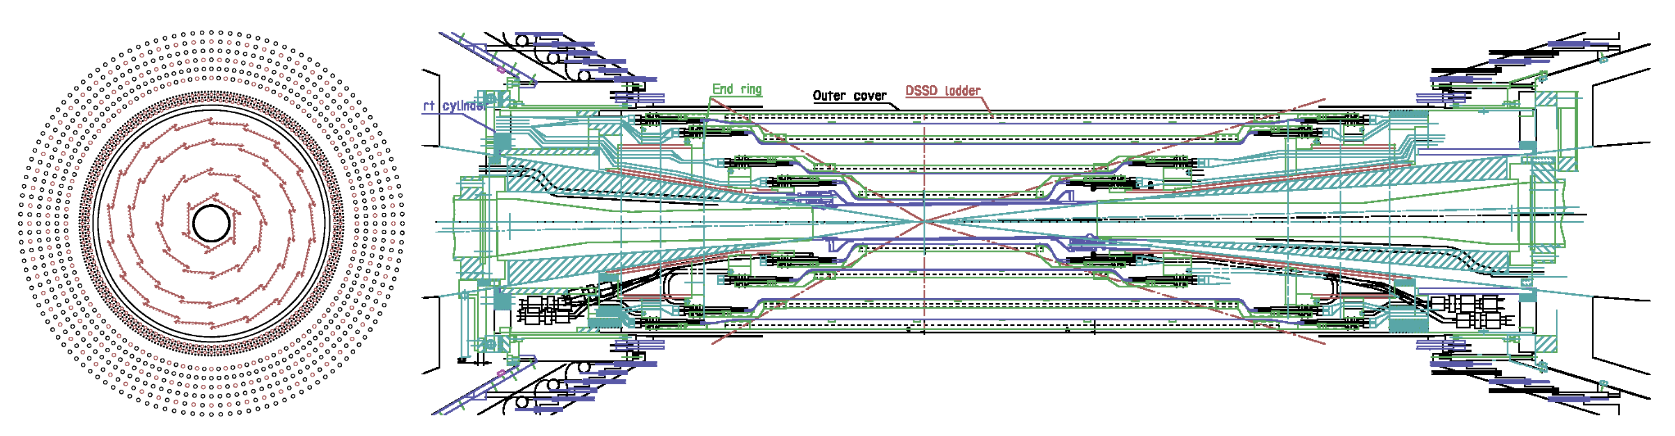
\includegraphics[width=\linewidth]{fig/setup/SVD_layout}
	\caption{Front (left) and side (right) view of the SVD detector with the SVD2 configuration. The front view also shows the inner wires of the
		Drift Chamber \cite{haba2004letter}.}
	\label{fig:SVD_layout}
\end{figure}

The efficiency of the SVD was determined as a fraction of CDC tracks within the SVD acceptance that have associated SVD hits, needed for the $B$ meson reconstruction. The average efficiency is found to be around $98\%$ and is in agreement with simulation. SVD performance is also determined via the impact parameter $z$ and $r\phi$ resolution, which was obtained from cosmic ray data. The momentum and angular dependence of the impact parameters is shown in Figure \ref{fig:SVD_performance} and is well represented by the following parametrization for the SVD2
\begin{align}
\sigma_z = 28\e{\mu m}\oplus \frac{32\e{\mu m}}{\left(p/(1\e{GeV}/c)\right)}\frac{1}{\beta \sin^{5/2}\theta},\\
\sigma_{r\phi} = 22\e{\mu m}\oplus \frac{36\e{\mu m}}{\left(p/(1\e{GeV}/c)\right)}\frac{1}{\beta \sin^{3/2}\theta},
\end{align}
where $p$ is the particle momentum, $\theta$ is the polar angle, and $\beta=v/c$. An advantage of the smaller distance between the IP and the first DSSD layer in SVD2 is clearly seen.

\begin{figure}[H]
	\centering
	\captionsetup{width=0.8\linewidth}
	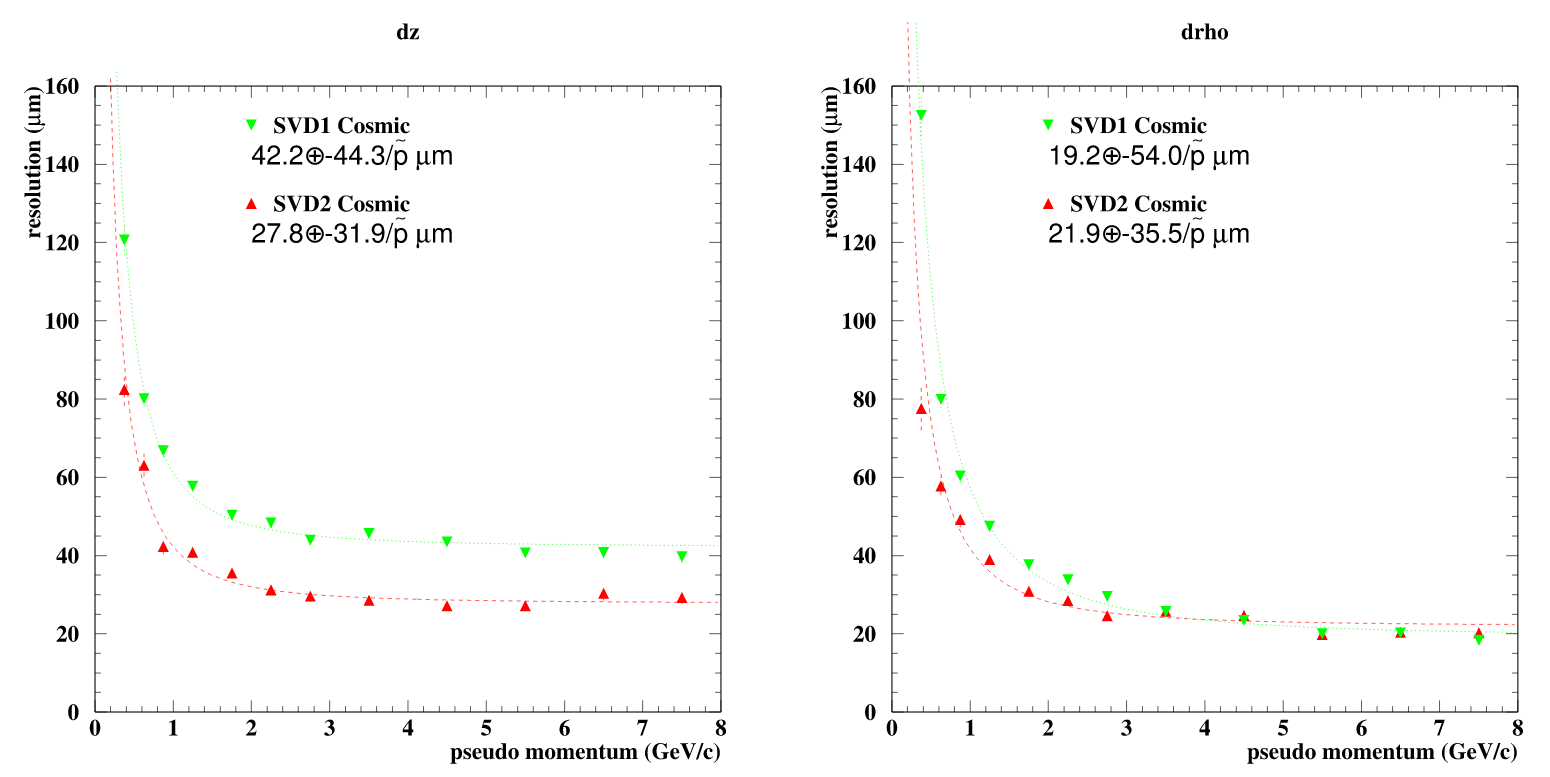
\includegraphics[width=\linewidth]{fig/setup/SVD_performance_1}
	\caption{Impact parameter resolutions of $z$ (left) and $r\phi$ (right) coordinates for the SVD1 and SVD2 configuration of the vertex detector \cite{haba2004letter}.}
	\label{fig:SVD_performance}
\end{figure}


\subsection{Central Drift Chamber}

CDC is a large-volume tracking device located at the central part of the Belle detector and is crucial for measurements of the particle trajectories and momenta, but also serves as a particle identification device (PID). It has a cylindrical structure with a radius of $88\e{cm}$, length of $2.4\e{m}$ and acceptance equal to the one of SVD2. The chamber has a total of $8400$ wires, which are positioned in $50$ layers and describe a nearly square wire configuration. There are two types of wires -- field wires for producing the electrical field, and sense wires for detecting the particles. Odd-numbered wire layers are oriented in the $z$ direction and provide a measurement of the transverse momentum $p_t$, while even-numbered wires are inclined with respect to the $z$ axis by a small angle of $\pm 50\e{mrad}$ to allow for measuring of the polar angle of the track. The wire configuration is shown in Figure \ref{fig:CDC_layout}. The space between the wires is filled with a gas mixture of $1:1$ helium-ethane, a low-$Z$ gas in order to minimize multiple-Coulomb scattering contributions to momentum resolution, since the majority of particles in $B$ events have a momentum lower than $1\e{GeV}/c$. It also has a small cross section of the photoelectric effect, which is important to reduce background electrons induced by the synchrotron radiation from the beam. 

\begin{figure}[H]
	\centering
	\captionsetup{width=0.8\linewidth}
	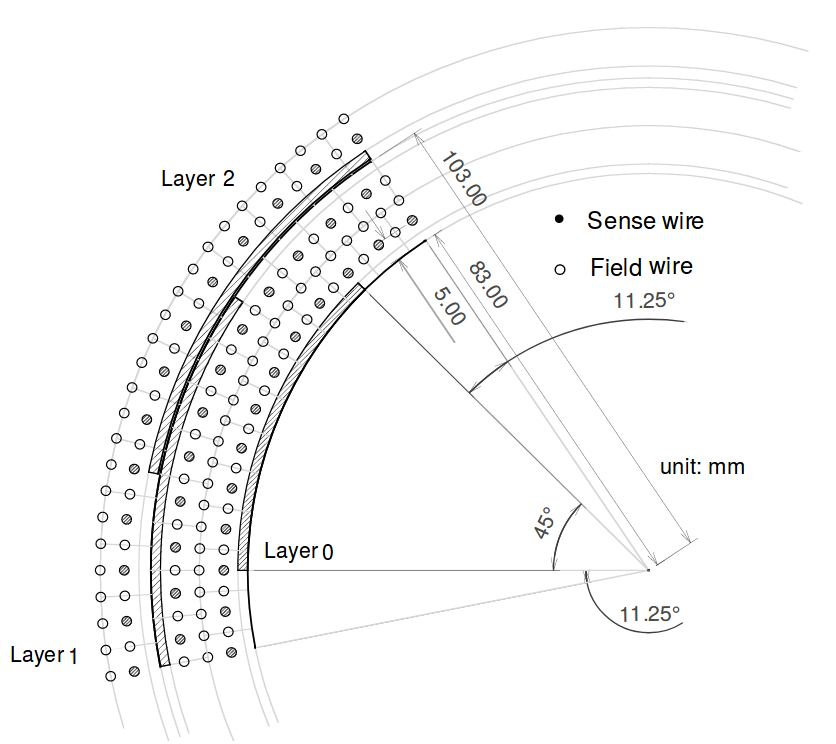
\includegraphics[width=0.6\linewidth]{fig/setup/CDC_layout}
	\caption{Cell structure of CDC \cite{ABASHIAN2002117}.}
	\label{fig:CDC_layout}
\end{figure}

Charged particles which pass the CDC wire frame cause gas ionization. The produced electrons drift toward the sense wires with great acceleration due to the strong electric field close to the wire. The accelerated electrons collide with gas molecules and produce secondary, tertiary etc. ionizations, which result in an electron avalanche, a process which increases the signal by many orders of magnitude. The primary electrons also have a specific drift velocity, which allows us to relate the measured pulse height and drift time to the energy deposit of the particle as well as the distance from the sense wire. This information is important for calculating the energy loss $\mathrm{d}E/\mathrm{d}x$. $\mathrm{d}E/\mathrm{d}x$ as a function of momentum differs for different particles, as shown in Figure \ref{fig:dEdx}. This allows for identification purposes of, specifically for kaons and pions. In the momentum region less than $0.8\e{GeV}/c$, $\mathrm{d}E/\mathrm{d}x$ enables a separation between kaons and pions up to $3\sigma$. The resolution of the transverse momentum measurement with the CDC is a function of the transverse momentum itself, as well as the particle velocity, and is parametrized as
\begin{equation}
\sigma(p_T)/p_T = \frac{0.201\%~p_T}{1\e{GeV}/c} \oplus \frac{0.290\%}{\beta}.
\end{equation}

\begin{figure}[H]
	\centering
	\captionsetup{width=0.8\linewidth}
	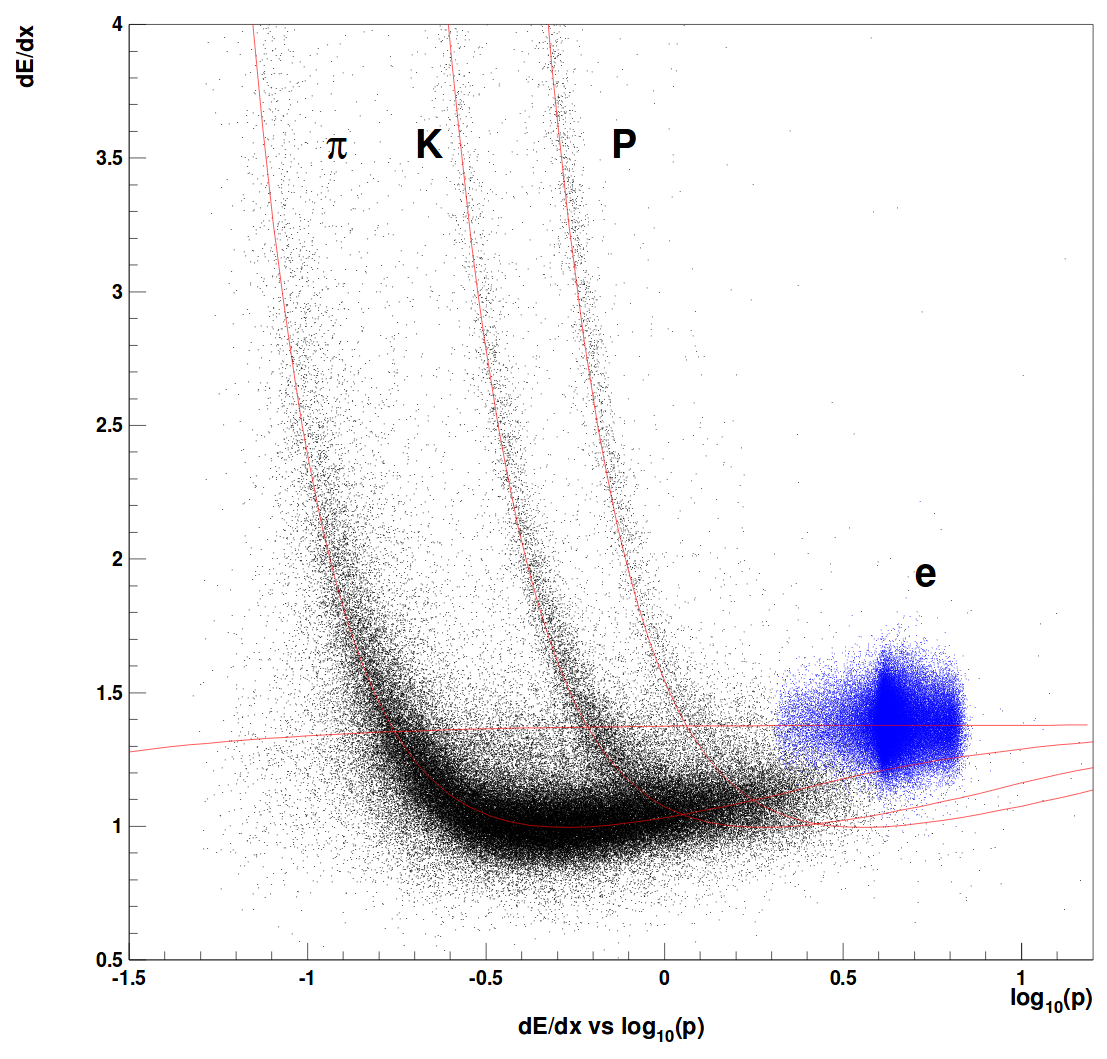
\includegraphics[width=0.6\linewidth]{fig/setup/dEdx}
	\caption{Measured $\mathrm{d}E/\mathrm{d}x$ as a function of particle momentum. The red lines show the expected distribution for different types of particles \cite{ABASHIAN2002117}.}
	\label{fig:dEdx}
\end{figure}

\subsection{Time-of-Flight Counter}

The purpose of the TOF subdetector is particle identification in the momentum region $0.8\e{GeV}/c < p < 1.2\e{GeV}/c$, especially for kaons and pions. There are 64 TOF modules in the barrel region, covering the polar angle of $33^\circ < \theta < 121^\circ$. One TOF module consists of two long polyvinyl toluene-based plastic scintillator bars, 4 fine-mesh photo-multiplier tubes (PMT) at the 4 ends of the bars, and a trigger scintillation counter, where the latter provides additional trigger information. TOF measures the time interval between the $e^+e^-$ collision and the passage of the particle through it. The mass of a particle can be inferred via the relation
\begin{equation}
m^2 = \left( \frac{1}{\beta^2}-1\right)p^2 = \left( \frac{T^2c^2}{L^2}-1\right)p^2,
\end{equation}
where $T$ is the measured time interval, $L$ is the charged particle trajectory length from the IP to TOF and $p$ is the charged particle momentum, determined by SVD and CDC. The resulting mass distribution for charged tracks measured by TOF in hadron events is shown in Figure \ref{fig:TOF_mass}, where clear peaks corresponding to pions, kaons and protons can be seen. To achieve the good discrimination between kaons and pions, a time-of-flight resolution of less than $100\e{ps}$ is needed for particles with momentum below about $1.2\e{GeV}/c$, which encompasses $90\%$ of the particles produced in $\Upsilon(4S)$ decays. The identification power can also be determined in the form of $\pi^\pm/K^\pm$ separation significance as a function of particle momentum, shown in Figure \ref{fig:TOF_separation}. A clear separation of about $2\sigma$ is achieved for particle momenta up to $1.25\e{GeV}/c$.

\begin{figure}[H]
	\centering
	\captionsetup{width=0.8\linewidth}
	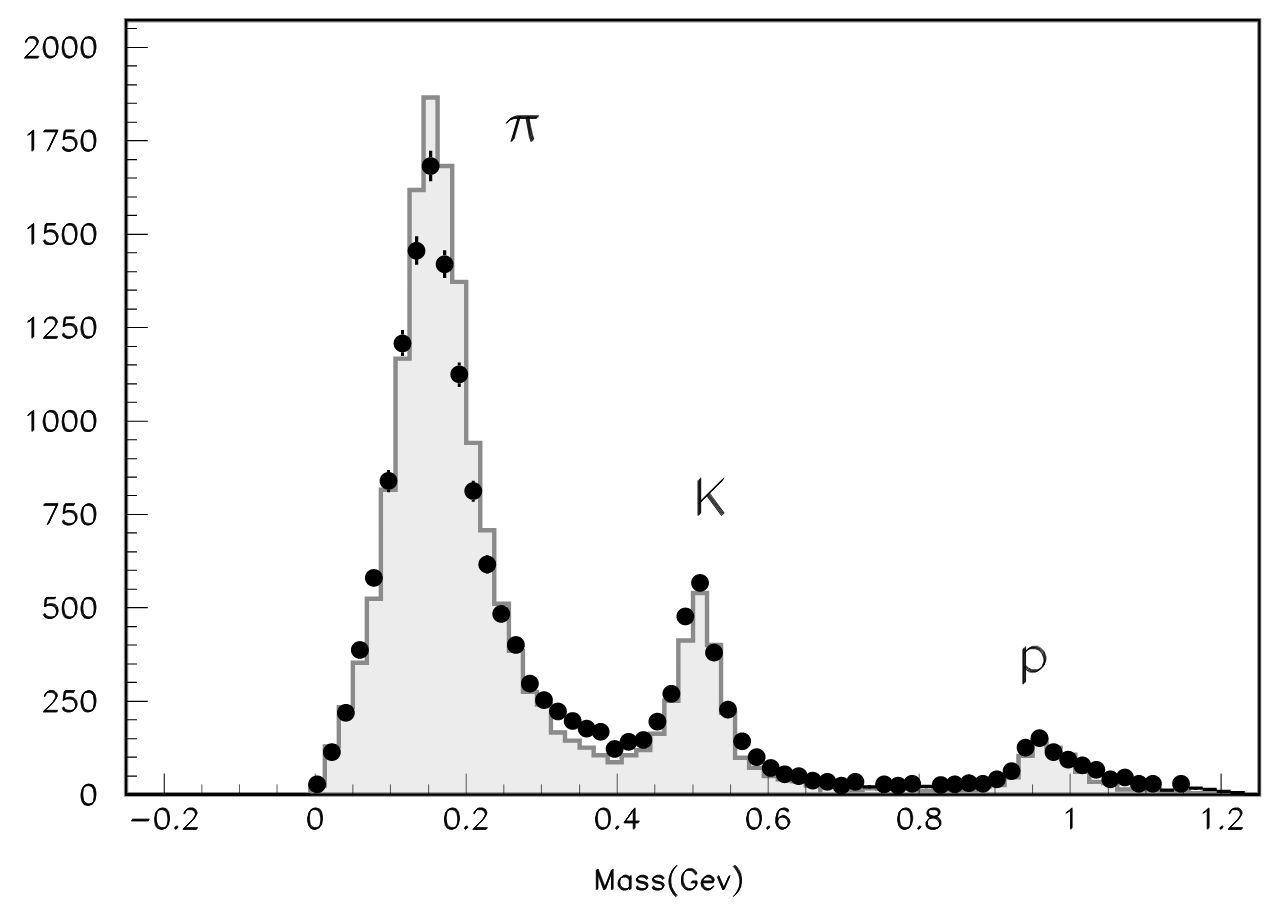
\includegraphics[width=0.6\linewidth]{fig/setup/TOF_mass}
	\caption{Mass distribution from TOF measurements for particle momenta below $1.2\e{GeV}/c$ \cite{ABASHIAN2002117}.}
	\label{fig:TOF_mass}
\end{figure}

\begin{figure}[H]
	\centering
	\captionsetup{width=0.8\linewidth}
	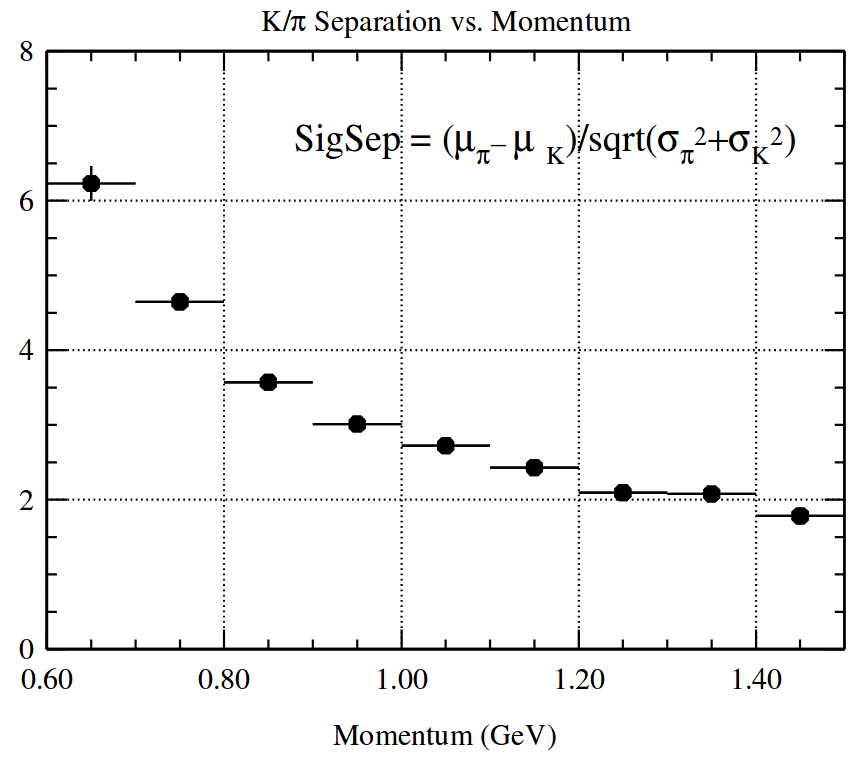
\includegraphics[width=0.6\linewidth]{fig/setup/TOF_separation}
	\caption{$\pi^\pm/K^\pm$ separation by TOF \cite{ABASHIAN2002117}.}
	\label{fig:TOF_separation}
\end{figure}


\subsection{Aerogel Cherenkov Counter}
TOF is not capable of performing good PID above $1.2\e{GeV}/c$ momentum since $\beta$ is almost equal to 1. For higher momenta in the region $1.0\e{GeV}/c < 4.0\e{GeV}/c$, the ACC is introduced. It is a threshold-type Cherenkov counter which utilizes the fact that particles emit Cherenkov light if the particle speed is greater than the speed of light in the passing medium. ACC is introduced in the barrel region with 960 separate modules, covering a polar angle of $34^\circ < \theta < 127^\circ$ and 228 modules in the forward end-cap region, with the polar angle coverage of $17^\circ < \theta < 34^\circ$. Each ACC module consists of an aluminum encased block of silica aerogel and one or two fine-mesh PMTs encased on each block to detect Cherenkov light pulses. Due to the polar angle dependence of the particle momentum, 6 different refractive indices are chosen for the aerogel material, ranging from $1.010$ up to $1.030$ and are controlled within $3\%$ precision. The layout of the ACC is shown in Figure \ref{fig:ACC_layout}.
\begin{figure}[H]
	\centering
	\captionsetup{width=0.8\linewidth}
	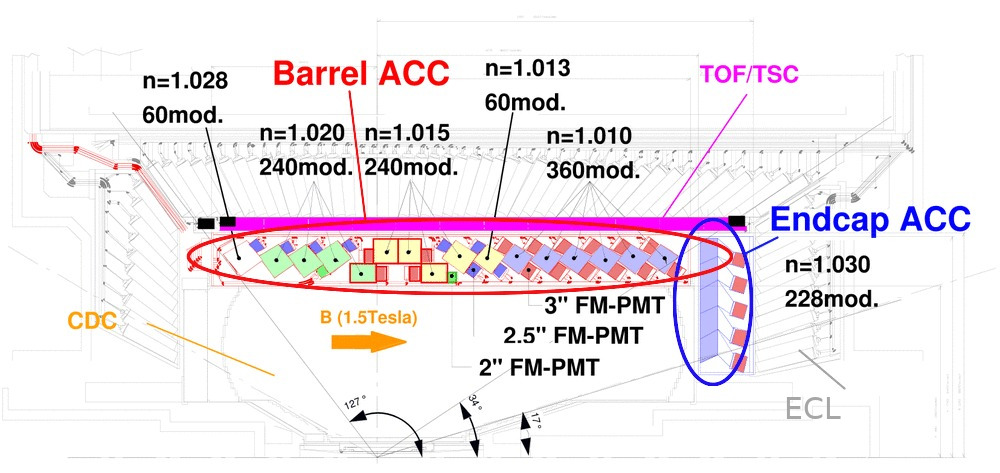
\includegraphics[width=\linewidth]{fig/setup/ACC_layout}
	\caption{Cross-sectional view of the CDC (inner most), ACC and TOF (outer most) detectors \cite{ABASHIAN2002117}.}
	\label{fig:ACC_layout}
\end{figure}
The threshold velocity $\beta$ of a given particle for Cherenkov radiation is
\begin{equation}
\beta \leq \frac{1}{n},
\end{equation}
where $n$ is the refractive index of the medium. The refractive indices in the ACC are such that, due to different masses, pions will emit Cherenkov light and kaons will not, due to different masses of the particles. Using the PID of ACC, along with other sub-system PID info, the electron identification efficiency in the momentum range above $1\e{GeV}/c$ is equal to or above $90\%$ while the pion fake rate, the probability of wrongly identifying pions as electrons, to be around $0.2$ - $0.3\%$. Similarly for kaons, kaon ID efficiency is equal to $80\%$ for most of the momentum region up to $4\e{GeV}/c$, while pion fake rate remains below $10\%$. Figure \ref{fig:ACC_eff} shows the electron and kaon efficiencies and the corresponding pion fake rates as a function of particle momenta.

\begin{figure}[H]
	\centering
	\captionsetup{width=0.8\linewidth}
	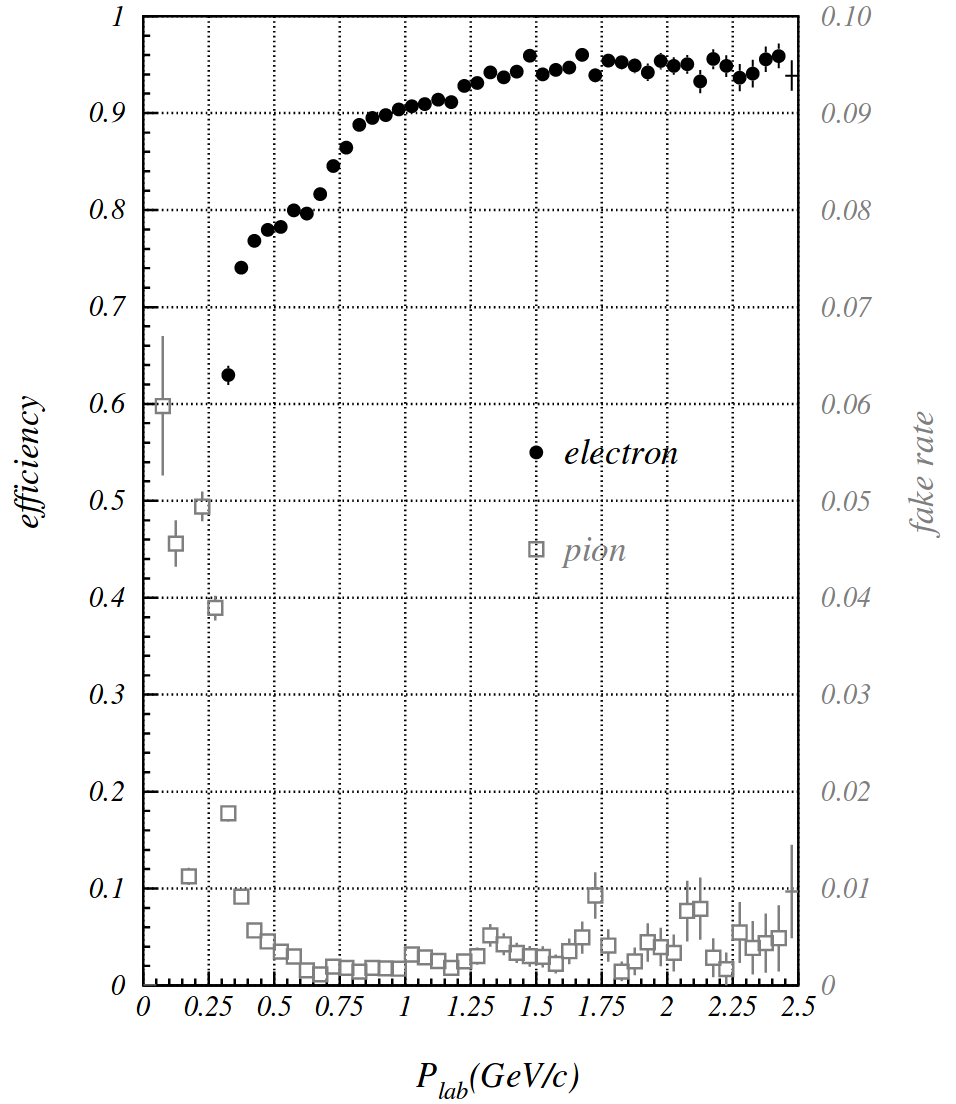
\includegraphics[width=0.48\linewidth]{fig/setup/ACC_eff1}
	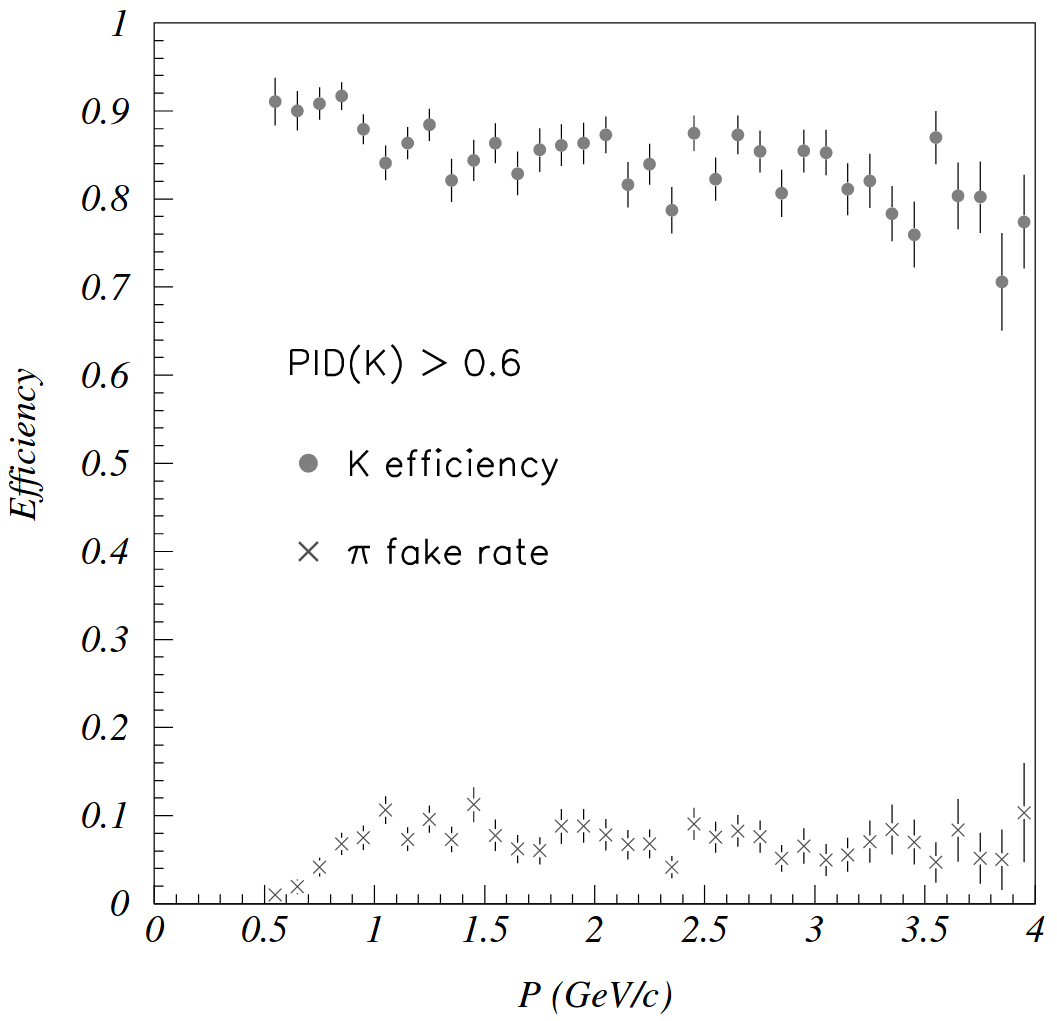
\includegraphics[width=0.48\linewidth,trim = 0cm -4cm 0cm 0cm]{fig/setup/ACC_eff2}
	\caption{Electron identification efficiency and fake rate for charged pions (left) and similarly for kaons (right). Note the different scales for the electron efficiency and fake rate in the former case \cite{ABASHIAN2002117}.}
	\label{fig:ACC_eff}
\end{figure}


\subsection{Electromagnetic Calorimeter}
Measurement of position and energy deposit of particles is performed in the ECL, especially for electrons and photons, where the latter are not measured by any of the subsystems described so far. It also provides complimentary particle identifications for electrons versus pions. The calorimeter consists of a highly segmented array of thallium-doped cesium iodide (CsI(Tl)) in the form of tower-shaped crystals, each pointing towards the IP. Each crystal is about $30\e{cm}$ long with a width from $44.5\e{mm}$ to $65\e{mm}$ in the barrel, and from $44.5\e{mm}$ to $82\e{mm}$ in the end-caps. Out of a total of 8736 crystals with a total mass of about $43\e{tons}$, 6624 of them are positioned in the barrel region and 1152 (960) in the forward (backward) end-caps. The inner radius of the barrel section is about $1.25\e{m}$, while the end-caps are positioned at $-1.0\e{m}$ and $2.0\e{m}$ from the IP in direction of the $z$ axis. The polar angle coverage of the barrel region is $32.2^\circ < \theta < 128.7^\circ$, and for the end-caps $12.4^\circ < \theta < 31.4^\circ$ and $130.7^\circ < \theta < 155.1^\circ$. Figure \ref{fig:ECL_layout} shows the layout of the barrel and end-caps ECL. 
\begin{figure}[H]
	\centering
	\captionsetup{width=0.8\linewidth}
	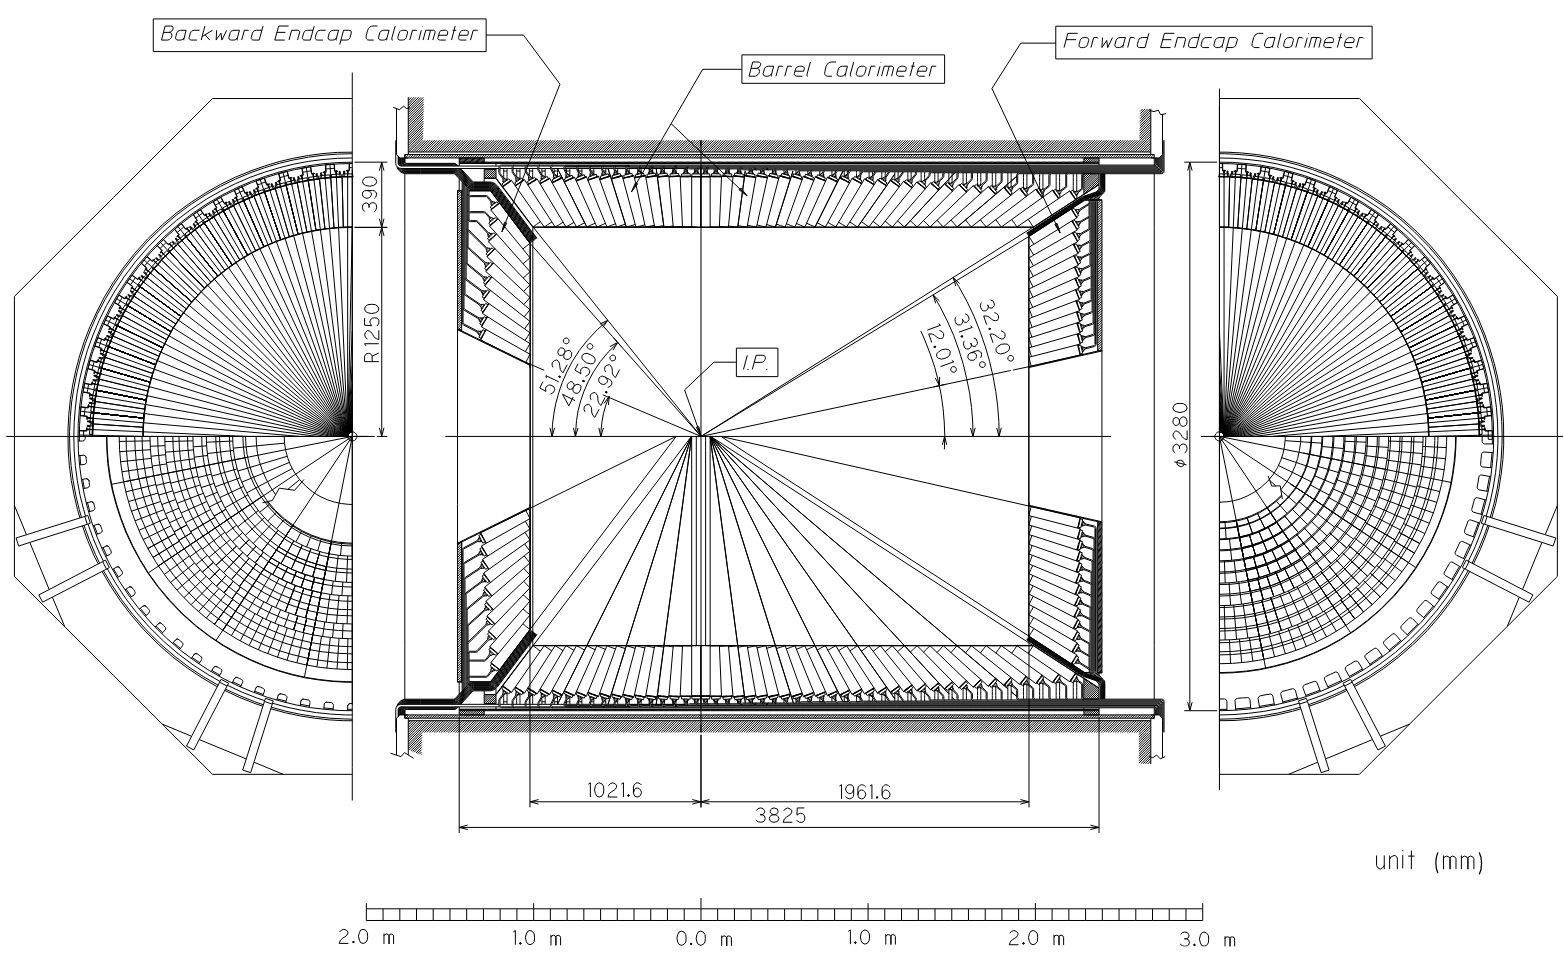
\includegraphics[width=\linewidth]{fig/setup/ECL_layout}
	\caption{Overall configuration of the ECL \cite{ABASHIAN2002117}.}
	\label{fig:ECL_layout}
\end{figure}
When an electron or a photon hits a crystal, it produces an electromagnetic shower, a result of the bremsstrahlung and pair-production effects. Heavier charged particles do not interact in the same way and deposit only a small amount of energy by ionization effects. The information from the ECL, compared with momentum measurements provided by the CDC, enables the identification of electrons. The distribution of the deposited energy for different particles is shown in Figure \ref{fig:ECL_deposit}. The probability of misidentifying an electron as a pion is approximately $5\%$ for momenta less than $1\e{GeV}/c$, and less than $1\%$ for momenta above $2\e{GeV}/c$.

\begin{figure}[H]
	\centering
	\captionsetup{width=0.8\linewidth}
	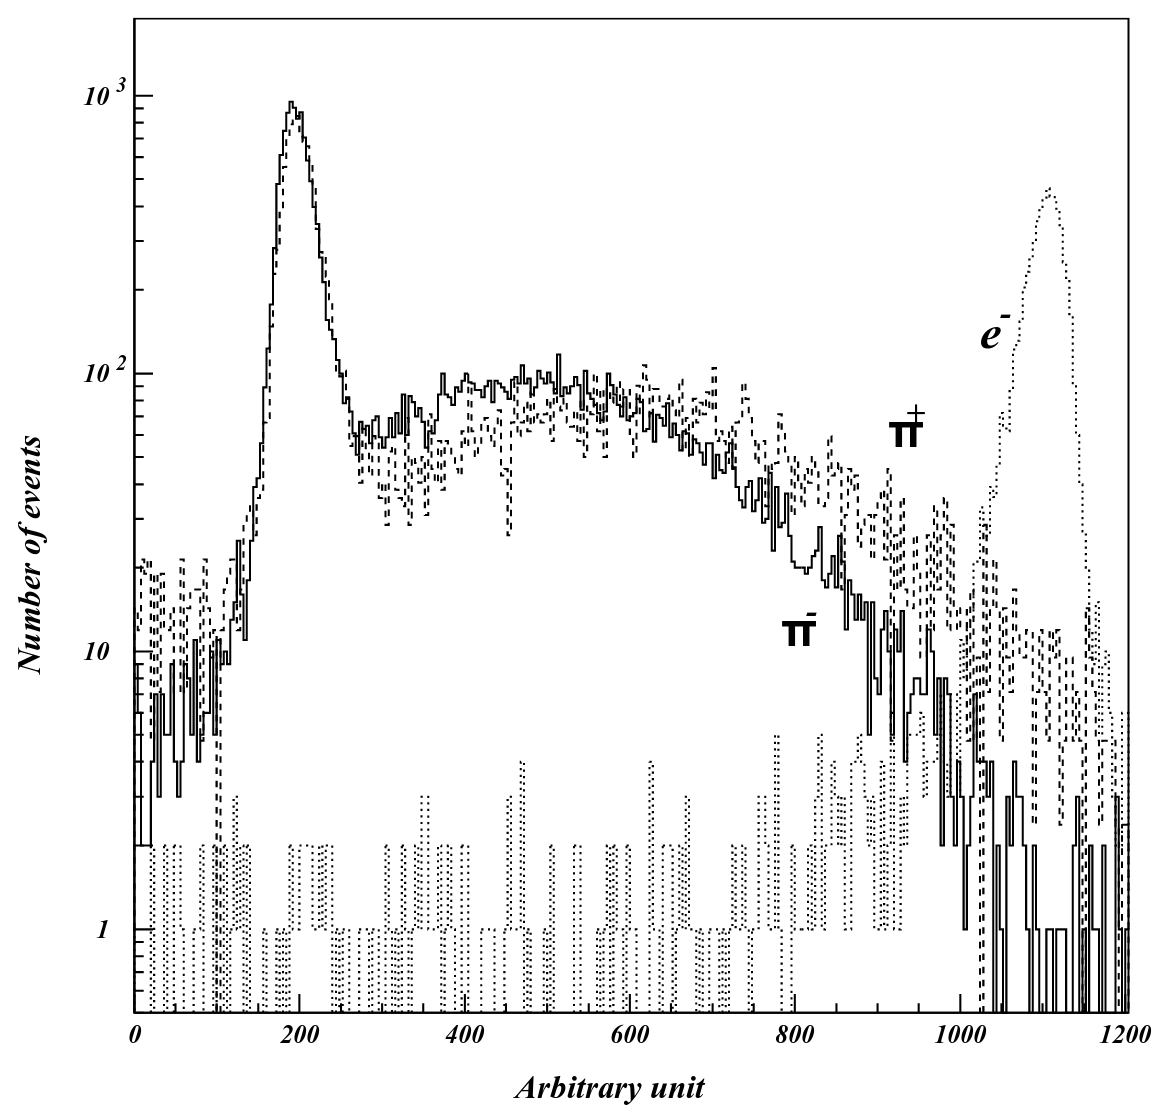
\includegraphics[width=0.6\linewidth]{fig/setup/ECL_deposit}
	\caption{Distribution of the energy deposit by electrons and charged pions at $1\e{GeV}/c$ momentum \cite{ABASHIAN2002117}.}
	\label{fig:ECL_deposit}
\end{figure}

For ECL calibration, $e^+e^- \to e^+e^-$ and $e^+e^- \to \gamma\gamma$ events were used. The average energy resolution was achieved to be $1.7\%$ for the barrel ECL, and $1.74\%$ and $2.85\%$ for the forward and backward ECL, respectively, as shown in Figure \ref{fig:ECL_resolution}. These value are in good agreement with Monte Carlo predictions. Worse energy resolution in backward end-cap is due to the lower photon energy, which results in larger effects of passive material in front of the calorimeter \cite{haba2004letter}. The energy resolution as a function of energy can be obtained via the following relation
\begin{equation}
\frac{\sigma_E}{E} = \frac{0.0066\%}{\left(E/1\e{GeV}\right)}\oplus\frac{1.53\%}{\left( E/1\e{GeV}\right)^{1/4}}\oplus 1.18\%,
\end{equation}
while the resolution of the position measurement is
\begin{equation}
\sigma_{pos} = 0.27\e{mm}+\frac{3.4\e{mm}}{\left( E/1\e{GeV}\right)^{1/2}} + \frac{1.8\e{mm}}{\left( E/1\e{GeV}\right)^{1/4}}.
\end{equation}

\begin{figure}[H]
	\centering
	\captionsetup{width=0.8\linewidth}
	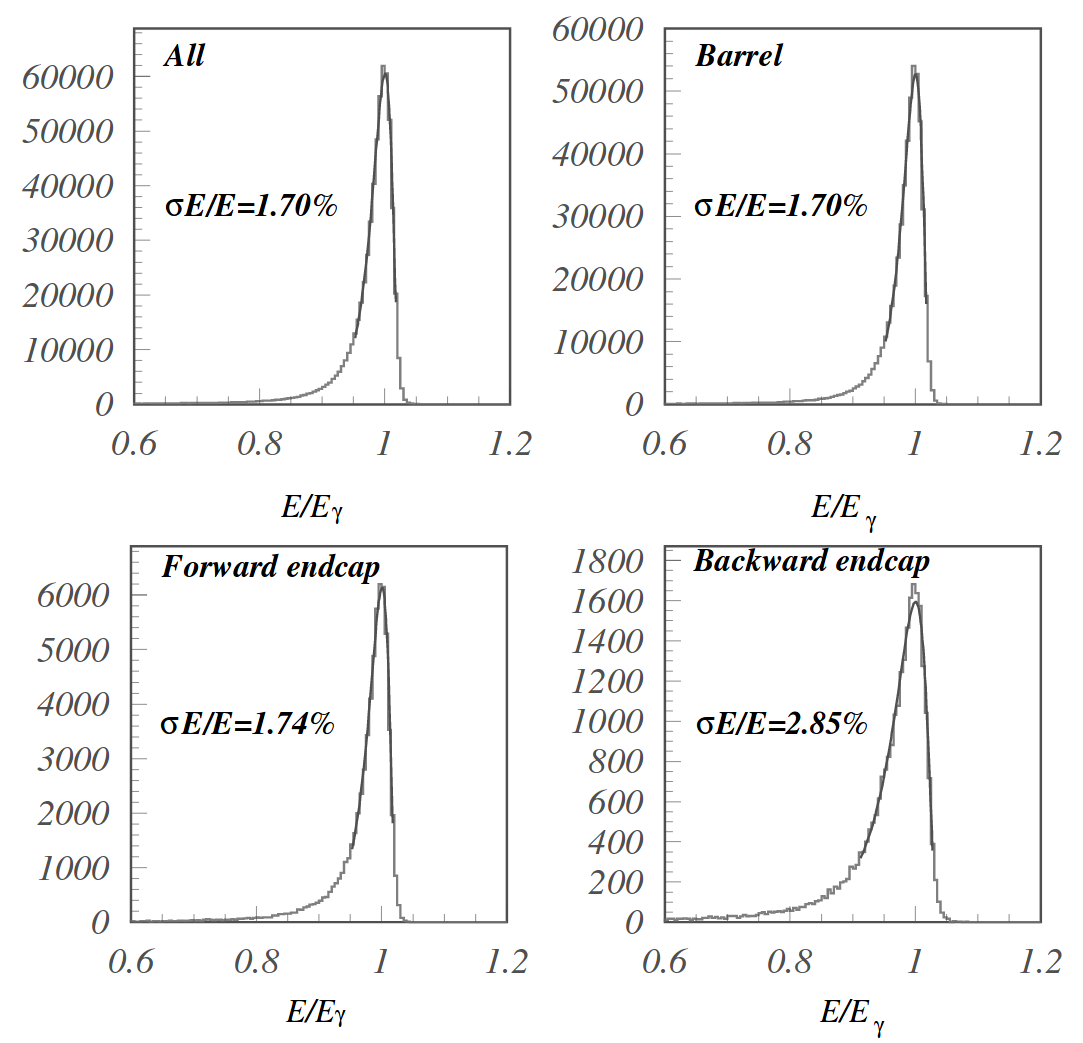
\includegraphics[width=0.8\linewidth]{fig/setup/ECL_resolution}
	\caption{Reconstructed energy distribution for $e^+e^- \to \gamma\gamma$ events for overall, barrel, forward and backward end-cap calorimeters \cite{ABASHIAN2002117}.}
	\label{fig:ECL_resolution}
\end{figure}

\subsection{$K_L^0/\mu$ Detector}
The KLM detector is used for detection of high-penetration particles such as $K_L^0$ and $\mu$ for momenta larger than $0.6\e{GeV}/c$. The setup covers the polar angle of $20^\circ < \theta < 155^\circ$. Detection of $K_L^0$ particles is troublesome since they are neutral and have a small material interaction probability, therefore a lot of material is needed in the KLM. To provide detection of both kinds of particles, hadronic and neutral, as well as electromagnetically and hadronically interacting, the KLM is constructed as a sampling calorimeter, which consists of 15 layers of $3.7\e{cm}$ thick resistive-plate counters (RPC) with 14 layers of $4.7\e{cm}$ thick iron plates between them. A single RPC module consists of two parallel plate electrodes, two glass panels, and gas in between. A charged particle passing the gas gap initiates a local discharge of the plates, which in turn induces signal to record the time and location of ionization. This is possible since the resistivity of the glass surface is high, so the discharge occurs locally. Hadrons interacting with the iron plates may produce a shower of ionizing particles, which are then also detected by the RPCs. The KLM is located outside of the superconducting solenoid and the iron plates of the KLM serve a dual role as the flux return for the magnetic field. Figure \ref{fig:KLM_layer} shows a cross-section of an RPC superlayer, consisting of an RPC pair.

\begin{figure}[H]
	\centering
	\captionsetup{width=0.8\linewidth}
	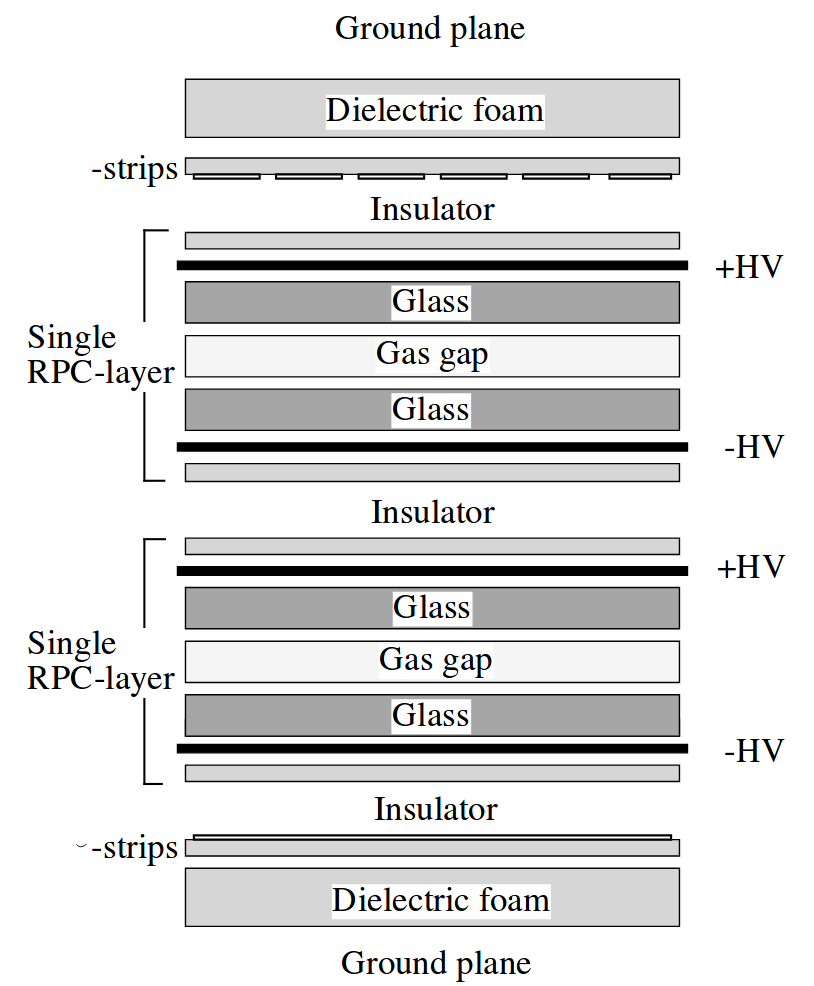
\includegraphics[width=0.4\linewidth]{fig/setup/KLM_layer}
	\caption{Cross-section of an RPC superlayer, consisting of an RPC pair \cite{ABASHIAN2002117}.}
	\label{fig:KLM_layer}
\end{figure}

The $K_L^0$ particle can be distinguished from other charged hadrons because they have no matched track in the CDC. The flight direction can also be inferred from the hit locations in the consecutive RPCs. Tracks of charged particles measured in CDC are extrapolated into KLM and clusters within $15^\circ$ of an extrapolated charged particle track are excluded from $K_L^0$ cluster candidates. On the other hand, muons with matched CDC tracks are able to reach the KLM if their momentum is larger than $0.5\e{GeV}/c$. They do not interact strongly and do not produce hadronic showers in the KLM, which serves as a handle on the muon identification. Figure \ref{fig:KLM_eff} (left) shows the number of neutral clusters per event and a Monte Carlo simulation of the predicted number of $K_L^0$ clusters per event. The average number of $K_L^0$ clusters per event is $0.5$. The agreement with the prediction gives us the confidence that the detector and our reconstruction software are performing correctly. Figure \ref{fig:KLM_eff} (right) shows the muon detection efficiency as a function of momentum and shown for a likelihood cut of $0.66$, where muon likelihood is based on the comparison of the measured range of a particle with the predicted range for a muon. Based on $K_S \to \pi^+\pi^-$ events, a muon identification efficiency of better than $90\%$ is determined,  with a pion fake rate of less than $5\%$ for particles with momenta more than $1.5\e{GeV}/c$ and a likelihood cut of $0.66$.

\begin{figure}[H]
	\centering
	\captionsetup{width=0.8\linewidth}
	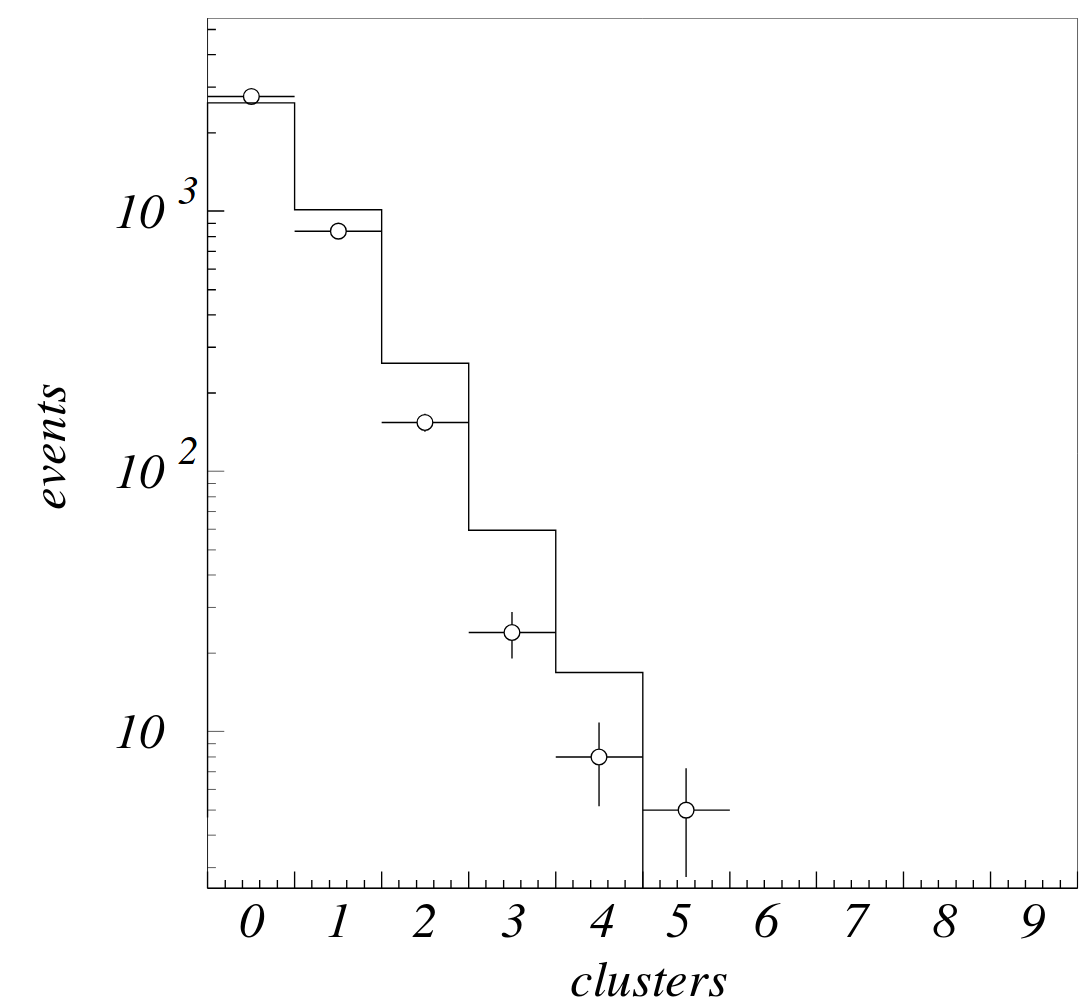
\includegraphics[width=0.48\linewidth,trim = 0cm -1.5cm 0cm 0cm]{fig/setup/KLM_clusters}
	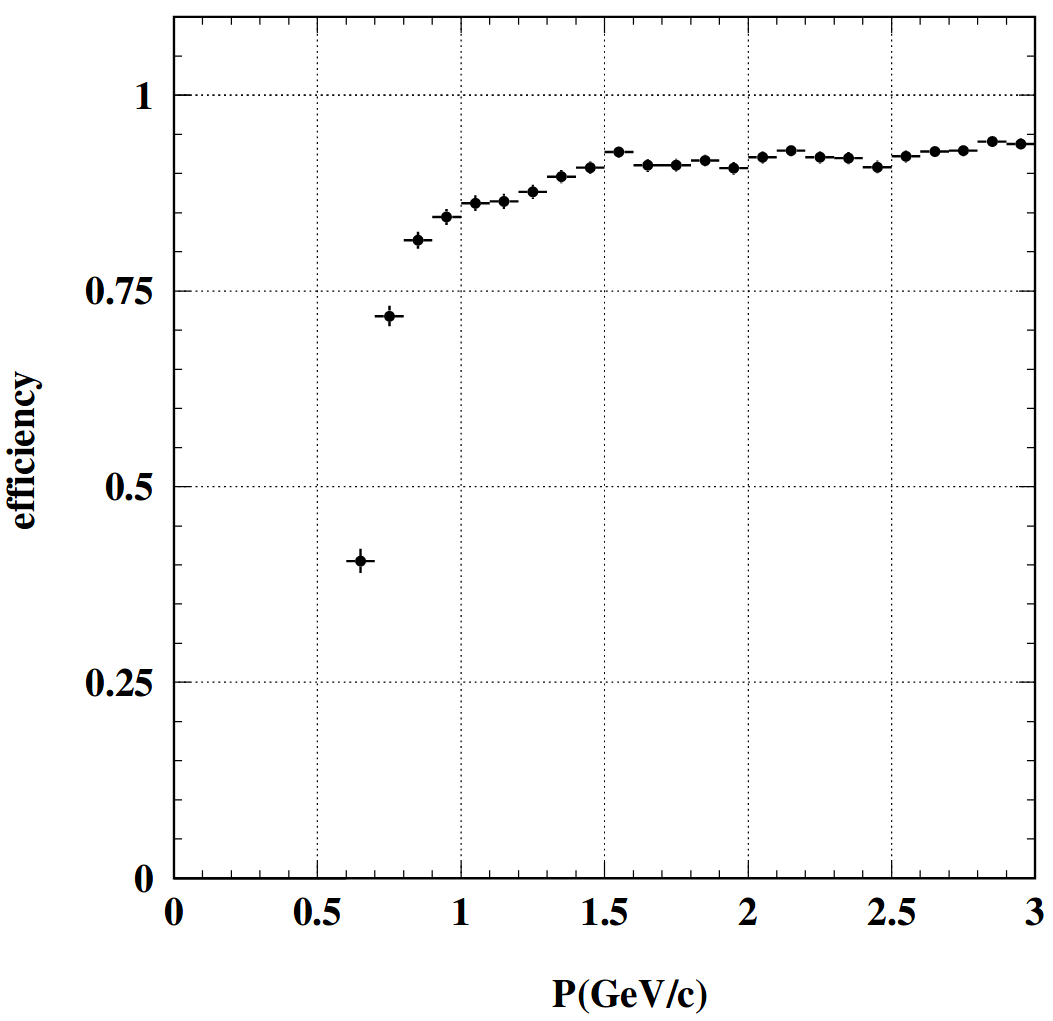
\includegraphics[width=0.48\linewidth]{fig/setup/KLM_efficiency}
	\caption{Number of neutral clusters per event in KLM (left) and muon detection efficiency as a function of momentum in KLM (right) \cite{ABASHIAN2002117}.}
	\label{fig:KLM_eff}
\end{figure}

Cosmic ray events have been used to determine the efficiency and resolution of the KLM, with an overall efficiency typically over $98\%$. The temporal and spatial resolutions of the KLM are few$\e{ns}$ and about $1.2\e{cm}$, respectively. The latter corresponds to an angular resolution from the interaction point of better than $10\e{mrad}$.

In order to do detector calibration and proper luminosity measurements, we need to accumulate samples of Bhabha and $\gamma\gamma$ scattering. Otherwise, as shown in Table \ref{tab:xsec}, the cross-section for physics events of interest is reasonably small. During normal operation (luminosity of $L = 10\E{34}\e{cm^{-2}s^{-1}}$) the total event rate is around $200\e{Hz}$, which is well below the data acquisition (DAQ) limit of $500\e{Hz}$. Out of this rate, $100\e{Hz}$ are physically interesting events, which include also two-photon events, Bhabha scattering, and $\mu$ pair production, besides hadronic events from $B \bar B$ pair events. In order to discard events which are not interesting for physics analyses, we use a trigger system by appropriately applying restrictive conditions. This section describes the necessary procedures and equipment to successfully do so.

\subsection{Trigger System}
The trigger system operates by immediately eliminating events that are not of interest, so that the amount of stored data is within the $500\e{Hz}$ frequency limit, while the efficiency for physics events of interest is kept high. Events which pass the triggers are then stored, otherwise discarded. The Belle trigger system consists of three stages, Level-1 (L1) online hardware trigger, Level-3 (L3) online software trigger and Level-4 (L4) offline software trigger.

L1 trigger is the first stage of the trigger system, which consists of multiple sub-detector triggers, all connected to a central trigger system called the Global Decision Logic (GDL), as schematically shown in Figure \ref{fig:TRG_GDL}. Each sub-detector trigger works on a principle of either a track trigger or an energy trigger. In the former case, the triggers discard events not meeting conditions based on the number of reconstructed tracks or track hits, while the latter is based on the total energy deposit and counting of crystal hits. Each sub-detector processes the event information and provides it to the GDL, where all the information is combined and the current event is characterized. The information from the sub-detector triggers reaches the GLD within $1.85\e{\mu s}$ after the collision, and the final trigger signal is provided within at a fixed $2.2\e{\mu s}$ latency. The combined efficiency from the L1 trigger is greater than $99.5\%$ for hadronic events.

\begin{figure}[H]
	\centering
	\captionsetup{width=0.8\linewidth}
	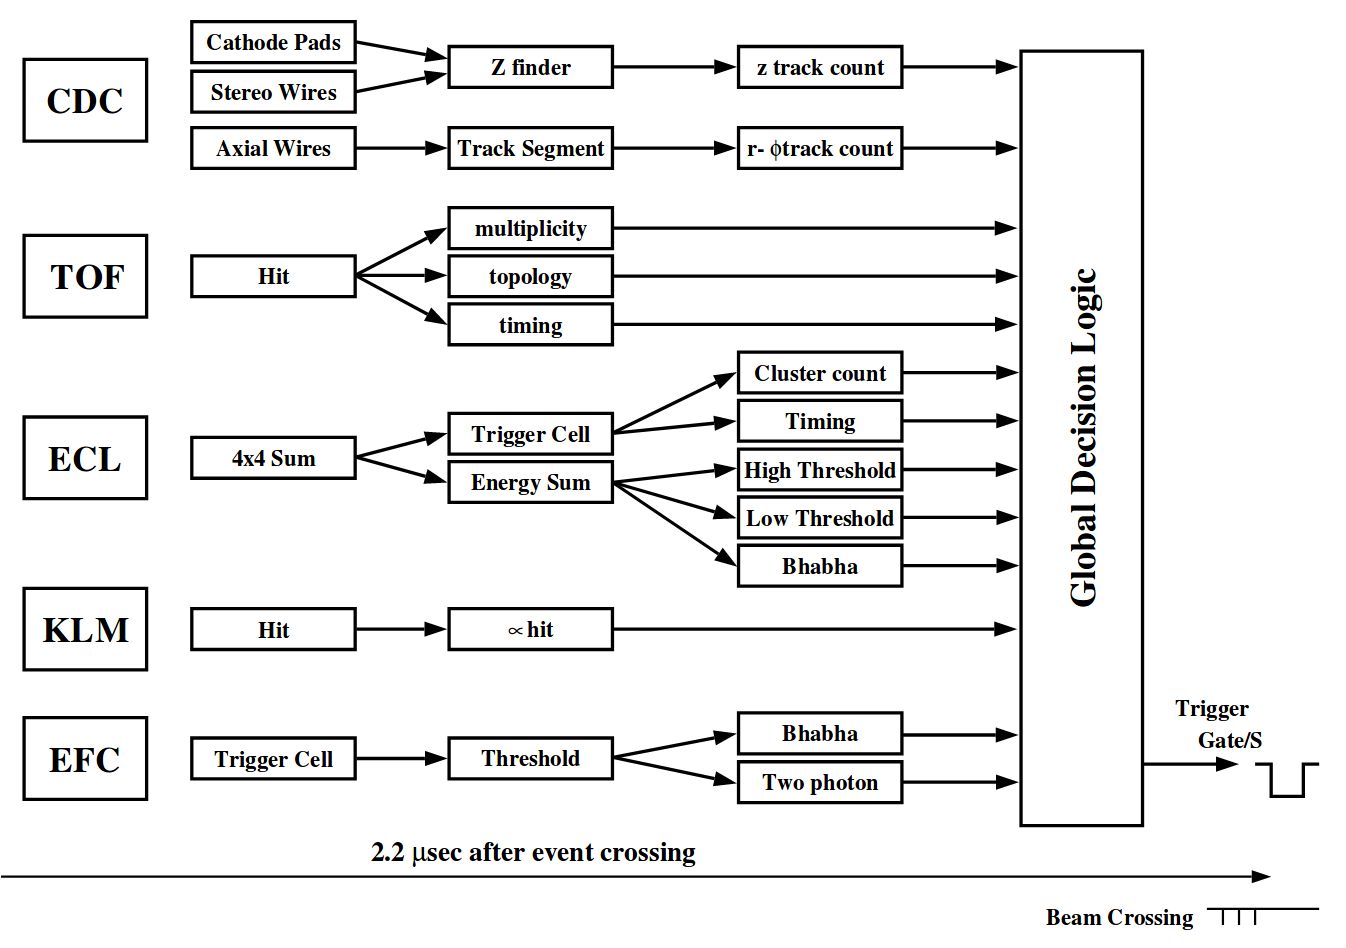
\includegraphics[width=0.8\linewidth]{fig/setup/TRG_GDL}
	\caption{The Level-1 trigger system for the Belle detector \cite{ABASHIAN2002117}.}
	\label{fig:TRG_GDL}
\end{figure}

After passing L1 trigger, the L3 discards background events from the software-wise perspective. L3 is an online software trigger which performs a simple, but fast reconstruction of the event. Events with at least one track satisfying the impact parameter condition $\vert\mathrm{d}z \vert < 5.0\e{cm}$ and with a total energy deposit in the ECL more than $1\e{GeV}/c$ are selected. The L3 trigger reduces the event rate by $50\%$, with a $99\%$ efficiency for hadronic events.

After passing the L3 trigger, the events are recorded on tapes. However, these data still contain many events from the beam background. To reduce the background events even further, they are required to pass the L4 offline software filtering. At the same time, high efficiencies for signal events is still required. Events must satisfy the following conditions
\begin{itemize}
	\item have at least one track with $p_T > 300\e{MeV}/c$ and impact parameters $\vert \mathrm{d}r \vert < 1.0\e{cm}$ and $\vert \mathrm{d}z \vert < 4.0\e{cm}$,
	\item have total energy deposit in the ECL must greater than $4\e{GeV}$.
\end{itemize}
Approximately $27\%$ of triggered events are passed through L4 while keeping an almost full efficiency for hadronic events. Events that pass the L4 trigger are fully reconstructed and stored to the DST. Overall, the efficiency of hadronic events after all trigger stages is measured to be more than $99\%$, which is more than the requirements from physics analyses.



